\section{\texorpdfstring{$\chi_{b1}$}{chib1} and \texorpdfstring{$\chi_{b2}$}{chib2} yields ratio}
\label{sec:ratio}

The ratio between $\chi_{b2}$ and $\chi_{b1}$ candidates is one of the parameters
in our fit model (Section~\ref{sec:chib:fit}). Nowadays this
ratio is estimated only in theoretical works, but recent
unpublished results with converted photons at \lhcb confirm these predictions.

In the recent theoretical work~\cite{Likhoded:2012hw} is shown
(Figure~\ref{fig:frac:ratio}) that the experimental results fo  cross section
and the transverse momentum distributions of the charmonium $\chi_{c1,2}$
states confirms the theory. 

\begin{figure}[H]
  \setlength{\unitlength}{1mm}
  \centering
  \begin{picture}(75,60)
    %
     \put(0,0){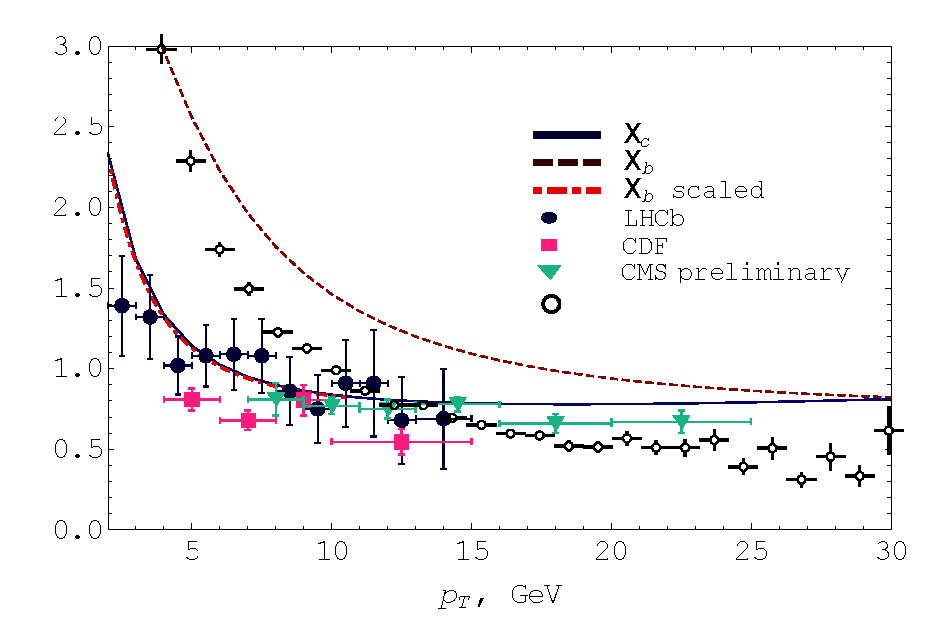
\includegraphics[width=75mm, height=60mm]{ratio/theory}}


     \put(-1,22){\begin{sideways}$\sigma({\chi_2})/\sigma({\chi_1}$)\end{sideways}}
     \put(46,30){\tiny $\chi_b$ scaled}
     \put(45,27){\tiny (this study, MC data)}

    % \graphpaper[5](0,0)(75, 60)
  \end{picture}
  \caption {\small This figure is taken from~\cite{Likhoded:2012hw} and shows
  transverse momentum distributions of the
$d\sigma\left[\chi_{2}\right]/d\sigma[\chi_{1}]$ ratio. Solid and dashed lines
stand for charmonium and bottomonium mesons. The dot-dashed line corresponds to
the rescaled bottomonium ratio:
$\sigma_{b2}/\sigma_{b1}(M_{\chi_c}/M_{\chi_b})\,p_T)$. The experimental results
for charmonium from LHCb \cite{LHCb-PAPER-2013-028} are shown with dots,
CDF~\cite{CDF:2007bra} --- with rectangles, and CMS~
\cite{CMS-PAS-BPH-11-010} --- with triangles. The scaled transverse momentum
distribution of \chib on Monte-Carlo data from this study is shown with open
circles. As it is seen, it almost matches the bottomonium curve. Thus the
results of this work have a reason to be used for fixing the fractions of
\chibone and \chibtwo yields on data. }
  \label{fig:frac:ratio}
\end{figure}

Since the result for bottomonium ratio could be obtained by rescaling the
charmonium curve, the  \chibone and \chibtwo ratio can be  measured by the
following formula in specified transverse momentum intervals of $\Upsilon$:
\begin{equation}
    \frac{N_{\chibtwo}^{data}}{N_{\chibone}^{data}} = \frac{\sigma(\chibtwo)}{\sigma(\chibone)}
    \frac{Br(\chibtwo\to\Upsilon\gamma)}{Br(\chibone\to\Upsilon\gamma)}\frac{\eps_{\chibtwo}^{\gamma}}{\eps_{\chibone}^{\gamma}}
\label{eqn:mc_ratio}
\end{equation}
\noindent where $\sigma(\chibtwo) / \sigma(\chibone)$ is a ratio
from~\cite{Likhoded:2012hw}, the branching fractions $Br(\chi_{b1,2} \to \Upsilon \gamma)$ 
are known experimentally~(\Cref{tab:branching}) and reconstruction efficiencies 
$\eps_{\chi_{b1,2}}^{\gamma}$ are obtained in this study~(\Crefrange{tab:mc:eff:chib1_y1}{tab:mc:eff:chib3_y3}).

\begin{table}[H]
\caption{The branching fractions of radiative \chibOneP and \chibTwoP mesons
decays are known experimentally~\cite{PDG2012}}
\centering
\begin{tabular}{l}
$Br(\chiboneOneP \to \Y1S \gamma) = 35\% \pm 8\%$ \\
$Br(\chibtwoOneP \to \Y1S \gamma) = 22\% \pm 4\%$ \\
$Br(\chiboneTwoP \to \Y1S \gamma) = 8.5\% \pm 1.3\%$ \\
$Br(\chibtwoTwoP \to \Y1S \gamma)  = 7.1\% \pm 1\%$ \\
$Br(\chiboneTwoP \to \Y2S \gamma) = 21\% \pm 4\%$ \\
$Br(\chibtwoTwoP \to \Y1S \gamma) = 16\% \pm 2.4\%$ \\
\end{tabular}
\label{tab:branching}
\end{table}

The $N_{\chibone}^{data}/(N_{\chibone}^{data} + N_{\chibtwo}^{data})$ ratio is
estimated by~\Cref{eqn:mc_ratio} to be in the range between 0.4 and 0.7 for
\chibOneP and \chibTwoP decays. The ratio for \chibThreeP decays could be
calculated because the branching fraction of these decays are unknown. In this
study this ratio is fixed to 0.5 and systematic uncertainty is assigned to this
decision.


% \begin{table}[H]
\caption{Summary of \chibone yield fraction ($\lambda_{\chi_{b1}(1,2P)}$)
determination  in data fits.}
\scalebox{0.6}{
	\begin{tabular}{lcccccccc}
	& \multicolumn8{c}{\OneS transverse momentum interval, \gevc} \\
	 & 6 --- 8 & 8 --- 10 & 10 --- 12 & 12 --- 14 & 14 --- 18 & 18 --- 22 & 22 --- 30 & 18 --- 30 \\
	\hline
	$\frac{\sigma{\chibtwo}}{\sigma{\chibone}}$  & 1.77 $\pm$ 0.17 & 1.50 $\pm$ 0.10 & 1.30 $\pm$ 0.10 & 1.15 $\pm$ 0.05 & 1.05 $\pm$ 0.05 & 0.95 $\pm$ 0.05 & 0.85 $\pm$ 0.05 & 0.90 $\pm$ 0.10 \\

	$\frac{\eps_{\chibtwo(1P)}}{\eps_{\chibone(1P)}}$  & 0.991 $\pm$ 0.013 & 1.029 $\pm$ 0.017 & 0.931 $\pm$ 0.019 & 0.970 $\pm$ 0.025 & 0.963 $\pm$ 0.028 & 1.03 $\pm$ 0.04 & 0.96 $\pm$ 0.05 & 1.003 $\pm$ 0.034 \\
	$\frac{\eps_{\chibtwo(2P)}}{\eps_{\chibone(2P)}}$  & 0.885 $\pm$ 0.015 & 0.873 $\pm$ 0.017 & 0.952 $\pm$ 0.021 & 0.978 $\pm$ 0.026 & 0.961 $\pm$ 0.032 & 1.00 $\pm$ 0.06 & 0.83 $\pm$ 0.07 & 0.95 $\pm$ 0.05 \\


	\rule{0pt}{4ex}$\frac{N_{\chibtwo(1P) \rightarrow \Y1S \gamma}}{N_{\chibone(1P) \rightarrow \Y1S \gamma}}$  & 1.11 $\pm$ 0.34 & 0.97 $\pm$ 0.29 & 0.76 $\pm$ 0.23 & 0.70 $\pm$ 0.21 & 0.64 $\pm$ 0.19 & 0.61 $\pm$ 0.18 & 0.51 $\pm$ 0.16 & 0.57 $\pm$ 0.18 \\

	$\frac{N_{\chibtwo(2P) \rightarrow \Y1S \gamma}}{N_{\chibone(2P) \rightarrow \Y1S \gamma}}$  & 1.31 $\pm$ 0.30 & 1.09 $\pm$ 0.24 & 1.03 $\pm$ 0.23 & 0.94 $\pm$ 0.20 & 0.84 $\pm$ 0.18 & 0.80 $\pm$ 0.18 & 0.59 $\pm$ 0.14 & 0.71 $\pm$ 0.17 \\

	\rule{0pt}{4ex}$\alpha_{\chiboneOneP}$  & 0.47 $\pm$ 0.08 & 0.51 $\pm$ 0.07 & 0.57 $\pm$ 0.07 & 0.59 $\pm$ 0.07 & 0.61 $\pm$ 0.07 & 0.62 $\pm$ 0.07 & 0.66 $\pm$ 0.07 & 0.64 $\pm$ 0.07 \\
	$\alpha_{\chiboneTwoP}$  & 0.43 $\pm$ 0.06 & 0.48 $\pm$ 0.05 & 0.49 $\pm$ 0.06 & 0.52 $\pm$ 0.05 & 0.54 $\pm$ 0.05 & 0.56 $\pm$ 0.06 & 0.63 $\pm$ 0.05 & 0.58 $\pm$ 0.06 \\
	\end{tabular}
}
\label{tab:ratio:lambda}
\end{table}

